\documentclass[12pt]{article}
\usepackage[a4paper, margin=2cm]{geometry}
\usepackage[english]{babel} % To obtain English text with the blindtext package
\usepackage{blindtext}
\usepackage{graphicx} % Required for inserting images
\usepackage{array, multirow} % For extra column formatting
\usepackage{amsmath, amssymb, cancel} %for equation environment
\usepackage{float}
\usepackage{parskip} % For gaps between para
\usepackage{setspace}
\usepackage{pdfpages}
\usepackage{abstract}
\usepackage[export]{adjustbox}
\usepackage{emptypage}
\usepackage{tocloft}
\usepackage[nottoc]{tocbibind}
\usepackage{hyperref, url}
\usepackage[table]{xcolor}
\usepackage{minted}
    \usemintedstyle{monokai}
\usepackage{caption}
    \captionsetup{font=footnotesize,labelfont=bf}
\usepackage{tcolorbox}
    \newtcolorbox{mintedbox}{
        colback=backcolour,
        boxrule=0pt,
        sharp corners,
        width=\linewidth,
        left=0pt, right=0pt,
        top=3pt, bottom=3pt
    }

\cftsetindents{section}{0em}{2em}
\cftsetindents{subsection}{0em}{2em}

\renewcommand\cfttoctitlefont{\hfill\Large\bfseries}
\renewcommand\cftaftertoctitle{\hfill\mbox{}}

\graphicspath{ {./images/} }

\pagenumbering{arabic}

\definecolor{blurple}{HTML}{5865F2}
\definecolor{backcolour}{HTML}{272823}

\hypersetup{
    colorlinks=true,
    linkcolor=black,
    urlcolor=blurple,
    citecolor=blurple,
}

\urlstyle{same}

\renewcommand{\arraystretch}{1.3}

\setcounter{secnumdepth}{5}
\setcounter{tocdepth}{5}
\newcommand\simpleparagraph[1]{%
  \stepcounter{paragraph}\paragraph*{\theparagraph\quad{}#1}}

%%%%%%%%%%%%%%%%%%%%%%%%%%%%%%%%%%%


\title{PHYC20040 Exp.2 Pleiades SM}
\author{Joana Adao}
\date{\today}

\begin{document}

\begin{titlepage}
    \begin{center}

        \begin{figure}[ht]
            
\includegraphics[width=\textwidth]{UCDLogo.png}
        \end{figure}
        
        \begin{figure}
            \centerline{
\includegraphics[width=\paperwidth]{UCDBanner.png}}
        \end{figure}

        \vspace{4cm}

        {\LARGE \bfseries PHYC20040 Exploring the Solar System}\\
        \vspace{0.75cm}
        {\Large Experiment No.2 Photoelectric Photometry of the Pleiades}
        
        \vspace{1cm}
    
    {\Large \textbf{12 February 2025}}

    \vspace{2cm}
    
    {\large \textbf{by Joana C.C. Adao (Student No. 23311051)}}\\

    \end{center}
    
   \clearpage

\end{titlepage}

\setcounter{page}{1}
\tableofcontents

\newpage

\begin{abstract}
\addcontentsline{toc}{section}{Abstract}

The aim of this experiment was to calculate the distance from Earth to the Pleiades star cluster using a CLEA (Contemporary Laboratory Experience in Astronomy) program to simulate the use of a photometer attached to a research telescope.
By finding the apparent magnitudes of 24 pre-selected stars through a Blue (B) and Visual (V) filter, the B-V colour index could then be calculated which ranged from \textbf{-0.11 to 1.70}. A plot of the visual apparent magnitude (m) was then plotted against the B-V values
for the Pleiades cluster and the line of the Main Sequence stars on the Hertzsprung-Russell diagram was overlaid on top it, with the absolute magnitudes (M) on the y-axis.

The distance modulus equation was then used with the values found to determine a distance of $\mathbf{410.4097 \pm 0.1955}$ \textbf{ly} from Earth to the Pleiades cluster. This result is \textbf{0.0999\%} off from
the estimated distance of 410 ly calculated in 1958 and \textbf{6.7251\%} off from the estimated distance of 440 ly calculated in 2004. These values were compared and verified against the accepted values and also compared against
the theoretical distance to the Sun if it were in the Pleiades cluster. Both distance modulus agreed at \textbf{0.55} indicating internal consistencies.

\end{abstract}

%%%%%%%%%%%%%%%%%%%%%%%%%%%%%%%%%%%

\vspace{4cm}

\section{Theory} \label{sec:1}

Photometry is an important technique in astronomy for measuring different properties of stars, such as brightness and temperature.
UBV Photometry and its consequent B-V colour index have greatly defined what it means to determine stellar classifications, leading to the development
of the H-R Diagram with a focus on main-sequence stars.

\subsection{Photometry} \label{sec:1.1}

\textbf{Photometry} is a measurement of the brightness of celestial objects, such as stars and planets, that give astronomers access to that celestial object's composition,
temperature, distance, age, and more
\cite{britphoto}.
It is a special subset of radiometry which measures light waves by the typical response of the average human eye
\cite{mictechphoto, photophoto}.

Photometry has some fundamental quantities that aid in understanding what is being measured \cite{WYATT197815,photophoto}:

\begin{itemize}
    \item \textbf{Luminous flux} is the visible light per second that the source radiates. It is measured with \textit{lumens} given by \textit{Watts}.
    \item \textbf{Luminous intensity}, directly related to the luminous flux, is the lumens per unit solid angle emitted. Originally known as 'candlepower', the unit of measurement
    is \textit{candela} given by \textit{Watts per steradian}.
    \item \textbf{Illuminance} is the measurement of the level of light at a particular surface. The unit of measurement is \textit{footcandle (English)} or \textit{lux (Metric)} which is
    given by \textit{Watts per square metre}.
    \item \textbf{Luminance} is what measures the apparent magnitude (brightness) (see §\ref{sec:1.1.3}), it is the luminous flux that is emitted from a surface.
    It is therefore measured with the unit \textit{footlambert (English)} or \textit{candela per square metre (Metric)}, given be \textit{Watt/steradian/}$m^2$.
    The human eye is the most commonly-known luminance detector, of which the sensitivity to light, and therefore colour, can be seen in figure {\ref{fig:1}}.
    \item \textbf{Luminosity} is a measure of the intrinsic brightness (absolute magnitude) of a star, measured in \textit{Watts}, mostly compared to the Sun's luminosity \cite{cosmoslumi}.
\end{itemize}

\begin{figure}[H]
    \centering
    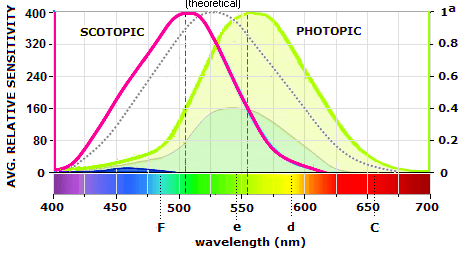
\includegraphics[width=12cm]{eye spectra curve.png}
    \caption{\centering Curve of the spectral sensitivity of the human eye \protect\cite{eyecurve}. \textit{Scotopic: very low light levels; Photopic: bright light levels \protect\cite{scophoto}.}}
    \label{fig:1}
\end{figure}

\subsubsection{UBV Photometry} \label{sec:1.1.1}

The UBV (Ultraviolet, Blue, Visual) classification system was originally called the Johnson-Morgan after H.L. Johnson and W.W. Morgan proposed this system for classifying stars in 1952 in accordance to their colour 
(and therefore temperature)
\cite{ubv1953}.
The apparent magnitudes of stars are measured in the three wavelength bands mentioned in section §\ref{sec:1.1} and their spectral types are determined through the associated B-V (blue filter) and U-B (Ultraviolet filter)
(\textit{the difference between the magnitudes through the different filters}) colour indices
\cite{ubv1953}.

\begin{figure}[H]
    \centering
    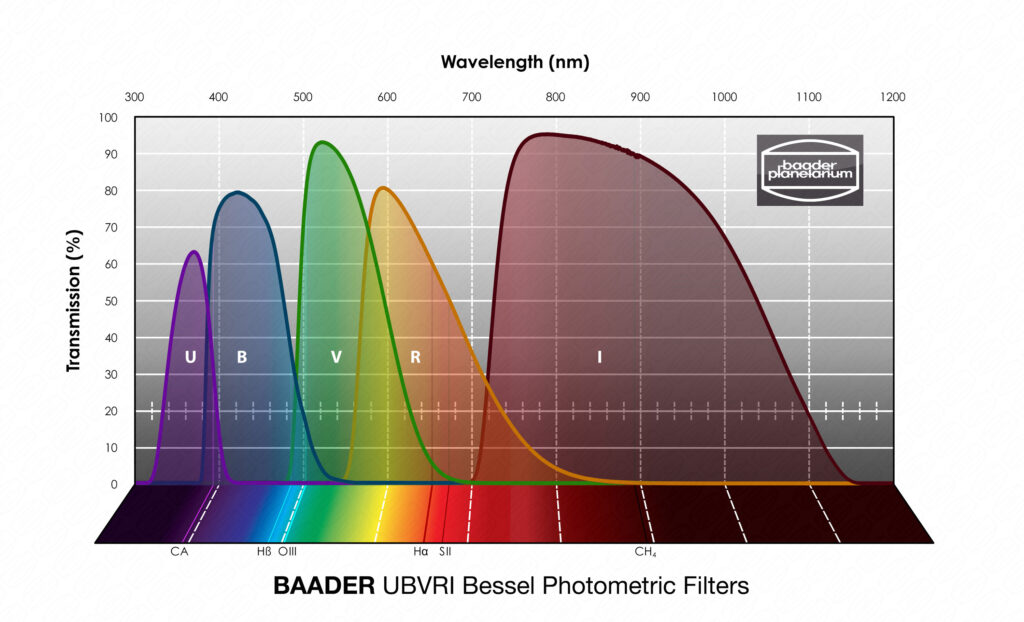
\includegraphics[width=12cm]{ubv.jpeg}
    \caption{\centering Transmission curves of photometric filters \protect\cite{ubvfilters}. \textit{U: Ultraviolet; B: Blue; V: Visible; R: Red; I: Infrared.}}
    \label{fig:ubvfilters}
\end{figure}

The UBVRI system in the above figure (\ref{fig:ubvfilters}) is an extension of the original Johnson-Morgan system with the extra red and infrared filters, allowing for a greater wavelength band allowance.

\subsubsection{The B-V Colour Index} \label{sec:1.1.2}

Colour, in astronomy, is defined as the difference in magnitude between two filters/wavelength bands, which is related to intensity logarithmically, 
\cite{sdsscolour,rochcolour,librecolour} such as B-V and U-B discussed in the previous section, §\ref{sec:1.1.1}.

On the flat, spanning z-axis of figure \ref{fig:ubvfilters} the B-V colour index (\textit{left}) that encompasses the range of visible light can be seen.

\subsubsection{Apparent and Absolute Magnitude} \label{sec:1.1.3}

Magnitude is a measure of the brightness of a star or other celestial body. The brighter the object, the lower the magnitude (number)
\cite{britmag}.
The magnitude of the celestial objects are divided into two types of observation:

\begin{itemize}
    \item \textbf{Apparent magnitude, m,} is used to describe how bright a celestial object appears from the view on Earth. Some of the brightest objects we can see
    have \textit{negative} apparent magnitude values (Sun = -26.7, Pluto (at brightest) = +13.7, for reference), meaning that they are particularly bright.
    \cite{lcomag}.
    \item \textbf{Absolute magnitude, M,} is defined as the magnitude of the star if the distance between it and Earth were 10 parsecs (pc)
    \cite{lcoabsmag,cosmosabsmag}.
    When at a set distance, astronomers are then able to compare intrinsic brightness of stars. The absolute magnitude refers to the absolute 'visual' magnitude, which restricts
    the measurement of the brightness to wavelength (4000 - 7000 Å)
    \cite{cosmosabsmag}.
    These magnitudes can also be negative values for particularly bright stars.
\end{itemize}

Absolute (\textbf{M}) and apparent (\textbf{m}) magnitudes can be used using equation \ref{eq:1} to calculate \textbf{D}, the distance in parsecs (pc). The magnitudes do not have units.
The distance modulus is then $\mathbf{m - M}$
\cite{cosmosabsmag}.

\vspace{-1.5ex}
\begin{gather} \label{eq:1}
    M = m + 5 - 5 (\log_{10} D) \quad , \quad m - M = 5 \log_{10} \left( \frac{D}{10} \right)
\end{gather}

The above equation (\ref{eq:1}) can be manipulated to find the distance, \textbf{D}:

\vspace{-1.5ex}
\begin{gather} \label{eq:2}
    \log_{10}D = \frac{m - M + 5}{5} \quad \implies \quad D = 10^{\frac{m - M + 5}{5}}
\end{gather}

\paragraph{The Link Between Magnitude and Photometry} \label{sec:1.1.3.1} has already been mentioned is sections §\ref{sec:1.1.1} and §\ref{sec:1.1.2}.

The zero point, a starting place for reference, was picked to be the star Vega, of which the magnitude is now defined to be $0.0$.
The apparent magnitudes are related to the flux of the star in such a way that equation \ref{eq:1} can be written to account for the flux (F) \cite{ccds}:

\vspace{-1.5ex}
\begin{gather} \label{eq:3}
    m_1 - m_2 = -2.5 \log_{10}\left(\frac{F_1}{F_2}\right) \qquad ; \qquad m_1 = -2.5 \log_{10}\left(\frac{F_1}{F_{Vega}}\right)
\end{gather}

Thus, the magnitudes can be interpreted as the logarithm of the flux.
Absolute magnitude, in contrast, is related to the luminosity (true brightness) of an object
\cite{ccds}.
The H-R Diagram, covered in §\ref{sec:1.2}, makes use of this relation.

\paragraph{The Link Between Magnitude and Colour} \label{sec:1.1.3.2} is what is explored further in this report.

The B-V colour index (see §\ref{sec:1.1.2}) is actually calculated by the difference in the apparent magnitudes as measured by the Blue (B) and Visual (V) filters
for the UBV photometric system \cite{ccds}:

\vspace{-1.5ex}
\begin{gather} \label{eq:4}
    B-V = m_B - m_V = -2.5 \log_{10}\left( \frac{f_B}{f_V} \right) + \text{constant}
\end{gather}

In which the non-zero constant is added due to the way the 0.0 colour (Vega) is defined. Thus is can be understood that bluer (hotter) stars have a negative colour
in comparison to Vega, and redder (colder) stars have a positive colour
\cite{ccds}.

\subsection{Hertzsprung-Russell (H-R) Diagram} \label{sec:1.2}

The Hertzsprung-Russell (H-R) diagram plots the absolute magnitudes (see §\ref{sec:1.1.3}) against the temperatures (spectral types) of different stars \cite{brithr}.
Figure \ref{fig:hrdiagram} also includes the luminosity (see §\ref{sec:1.1}) and B-V colour (see §\ref{sec:1.1.2}) as axes on the graph.
The 0.0 base point of the star Vega as discussed in sections §\ref{sec:1.1.3.1} and §\ref{sec:1.1.3.2} is included to the far left of the bottom y-axis.

\begin{figure}[H]
    \centering
    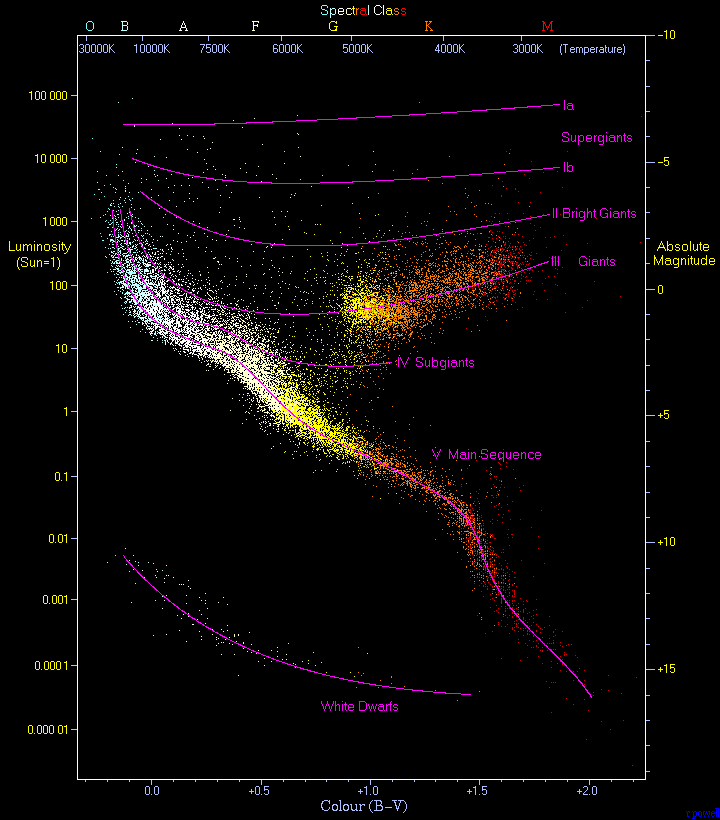
\includegraphics[width=10cm]{HRDiagram.png}
    \caption{\centering The Hertzsprung-Russell Diagram with 22 000 stars plotted in different regions highlighted accordingly \protect\cite{wikihr}.}
    \label{fig:hrdiagram}
\end{figure}

Astronomers can then use this diagram to be able to understand a star's internal structure and composition by determining its position on it \cite{cosmoshr,brithr}.
The way in which the stars scattered along the H-R diagram allowed astronomers to dictate the different regions, with the Main Sequence stars running diagonally across as
the most prominent and the gaints clustered above them in the diagram \cite{lcohr,cosmoshr}.

\subsubsection{Spectral Types} \label{sec:1.2.1}

The currently-used system of classification of stars was created by a team at Harvard in 1924 \cite{harvardstar}. The different classes are \textbf{OBAFGKM}, left to right: hottest to coldest.
The different classes and temperature thresholds are illustrated in figure \ref{fig:starclassy} with additional relevant information such as the (absorption) spectrum, the star colour, amount of hydrogen present, 
size in solar radii, and their prevalence (in percent) among the main sequence stars (see §\ref{sec:1.2.2})
\cite{lcostar,cosmosstar}.

\begin{figure}[H]
    \centering
    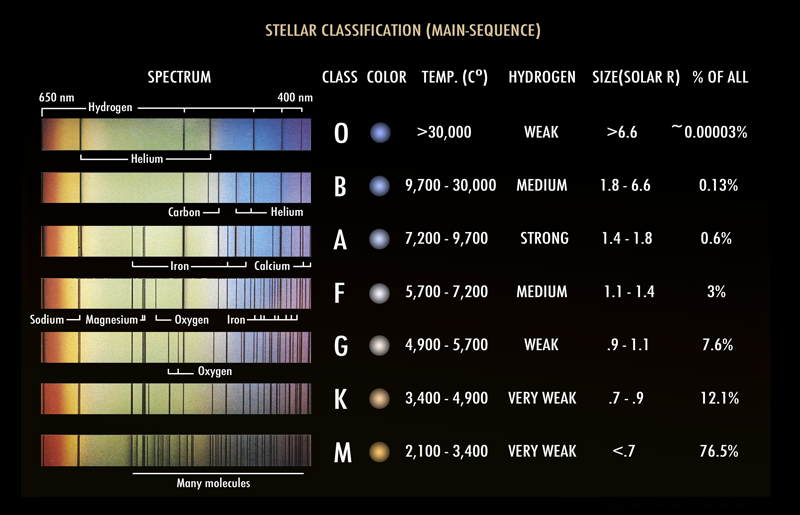
\includegraphics[width=.9\textwidth]{Stellar_Classification_Chart.png}
    \caption{\centering Chart for classifying of the main star types as per the Harvard classification \protect\cite{wikistar}.}
    \label{fig:starclassy}
\end{figure}

The Sun is spectral type \textbf{G2} with temperature 5 700 K (Kelvin) \cite{cosmosstar}.

\subsubsection{Main Sequence Stars} \label{sec:1.2.2}

Main sequence stars are stars that undergo the fusion of hydrogen into helium at their core through nuclear reactions
\cite{schoolmsstar,studymsstar,nasamsstar}.
They are also defined by the way the radiation pressure from the nuclear reactions and the gravitational pressure work against each other in such a way that the star
remains stable \cite{studymsstar}; the process is known as \textbf{hydrostatic equilibrium} \cite{schoolmsstar}.

The relationship of a main sequence star with luminosity and temperature (spectral type) is seen in figure \ref{fig:hrdiagram}, the H-R diagram, and figure \ref{fig:starclassy},
the stellar type classification (for main sequence stars), which also shows the hydrogen available to undergo the nuclear reactions into helium.

\subsection{The Pleiades Star Cluster} \label{sec:1.3}

The Pleiades star cluster, also known as \textit{the Seven Sisters} and \textit{Messier (M) 45} and \textit{Cl Melotte 22}, can be found and seen by the naked eye near the shoulder of the Taurus (bull) constellation during Winter
\cite{nasapleiades,hubblepleiades}.
It is an open star cluster, in such that it contains thousands of stars that are loosely bound by gravity \cite{nasapleiades}.

Hubble telescope's Fine Guidance Sensors have estimated that the distance to the Pleiades from Earth is about \textbf{440 light-years} \cite{hubblepleiades} 
with an apparent magnitude of \textbf{1.6} \cite{sedspleiades,frenchpleiades}.

\begin{minipage}{.43\textwidth}
    \captionsetup{hypcap=false}
    \centering
    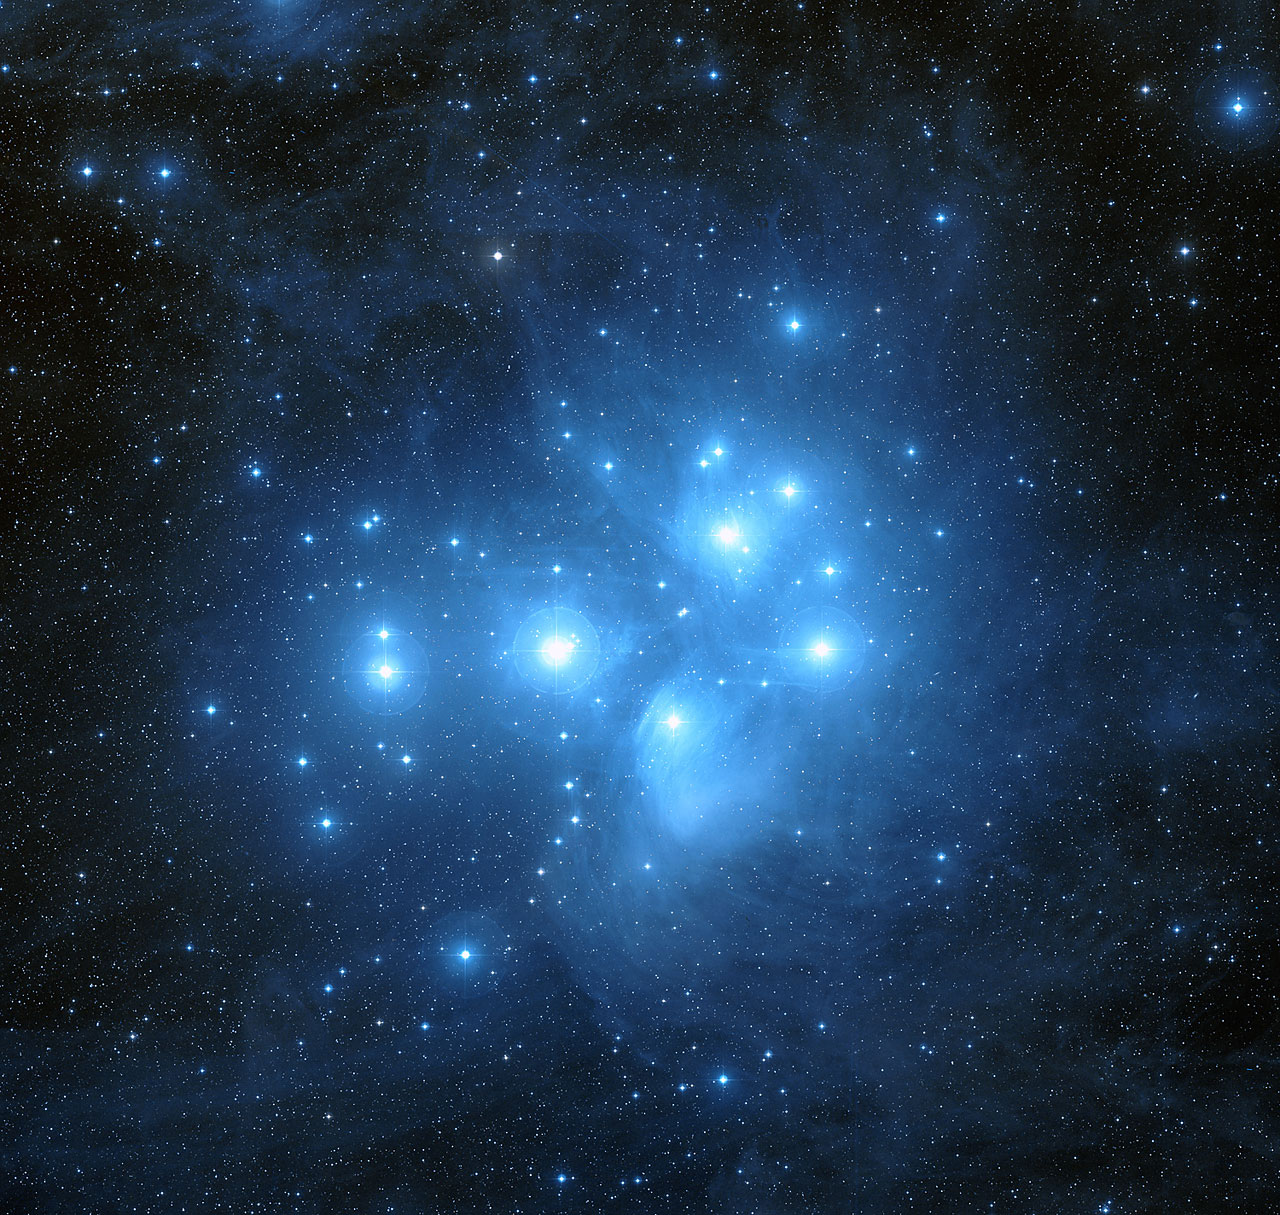
\includegraphics[width=\linewidth]{pleiades.jpg}
    \captionof{figure}{\centering Photo of the Pleiades/M45 \protect\cite{pleiades}.}
    \label{fig:plei}
\end{minipage}
\hfill
\begin{minipage}{.56\textwidth}
    \captionsetup{hypcap=false}
    \centering
    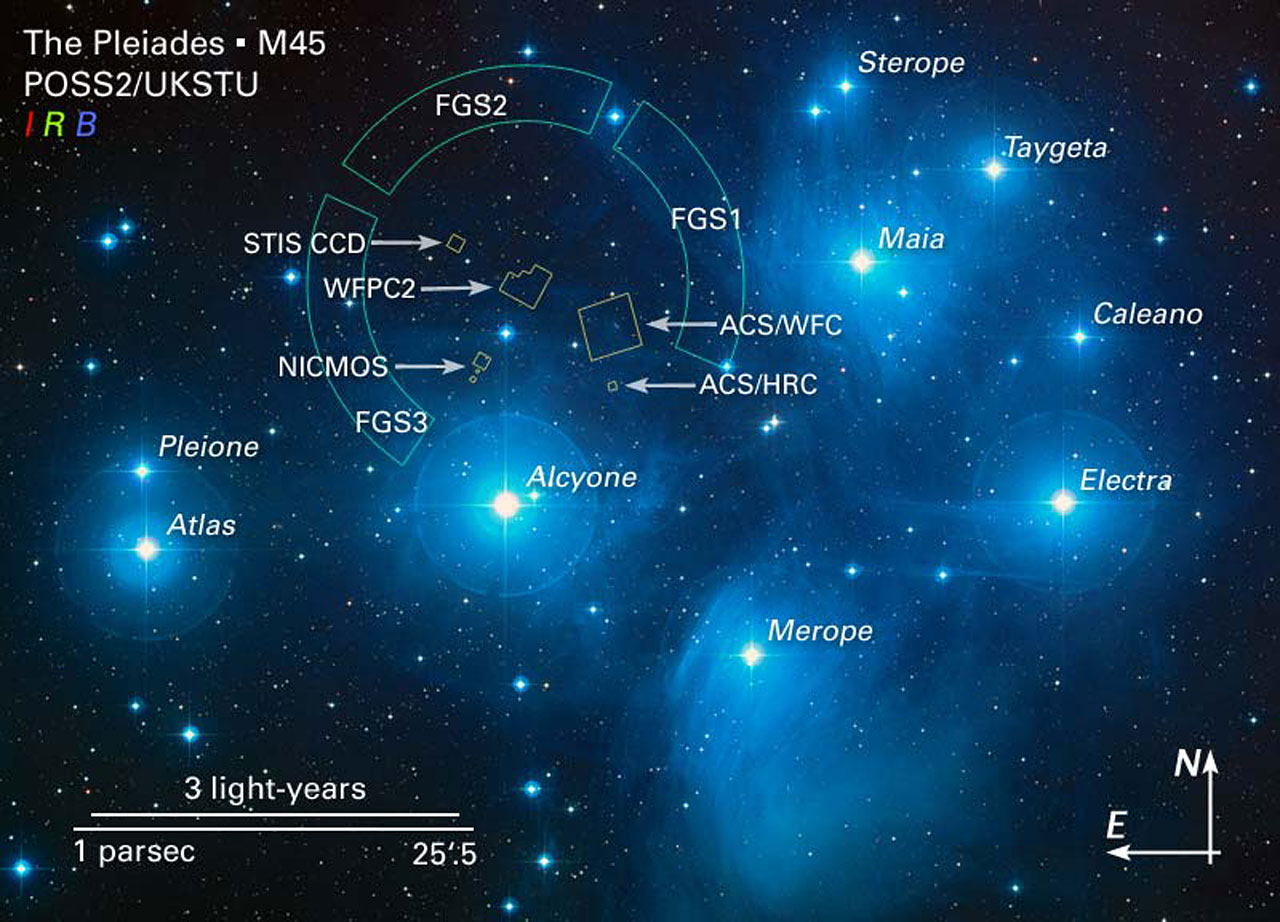
\includegraphics[width=\linewidth]{pleiades anotated.jpg}
    \captionof{figure}{\centering Annotated photo of the Pleiades/M45 \protect\cite{pleiadesann}.}
    \label{fig:pleiann}
\end{minipage}

Figure \ref{fig:plei} and figure \ref{fig:pleiann} are images sourced from the Hubble telescope of the Pleiades star cluster, with figure \ref{fig:pleiann} having the most visible stars named and labelled
and the Fine Guidance Sensors shown at the periphery of Hubble's field-of-view, tracing the circumference that is the approximate angular size of the Moon \cite{pleiadesann}.
A size/distance scale is also seen in the bottom left corner.

\begin{figure}[H]
    \centering
    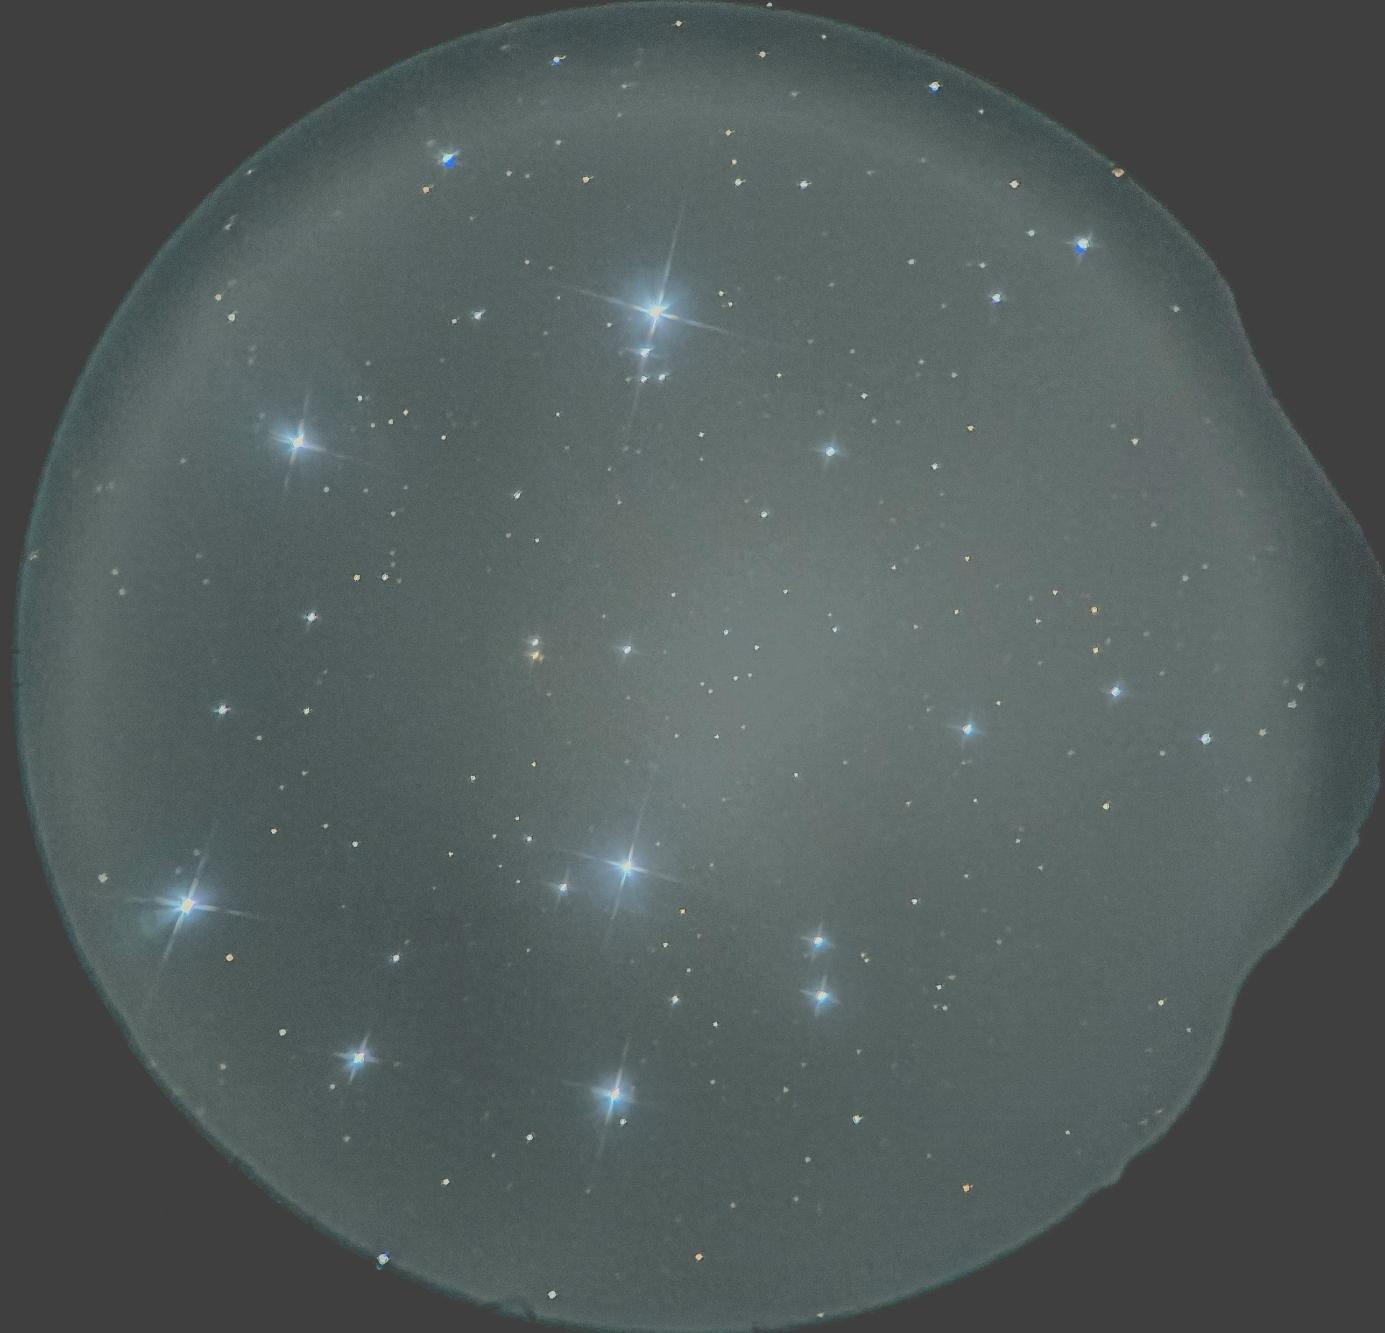
\includegraphics[width=7.5cm]{rian pleiades.jpg}
    \caption{\centering Image of the Pleiades as taken from a telescope \protect\cite{rian}.}
    \label{fig:visibleplei}
\end{figure}

A photo of the Pleiades star cluster taken through the view of a telescope (photographed by fellow Rian Byrne)\cite{rian} can serve as an example of the view of this star cluster through the V (Visual) lens.

\section{Methodology} \label{sec:2}

This experiment made use of the \textit{Contemporary Laboratory Experience in Astronomy}, CLEA, software and the \textit{Photoelectric Photometry of the Pleiades} program included in the package.
CLEA is an online software developed to simulate and illustrate modern astronomical techniques in a 'real' night sky
\cite{cleasm}.

The program offered the simulated use of a UBV photometer attached to a 0.4m (16") research telescope. As the Earth rotates to the East in the program, the available "tracking" feature is used to essentially "stop"
the movement of the stars (West) in relation to the rotation of the Earth, allowing for the stable collection of data.

The apparent magnitude for two filters, Blue (B) and Visual (V), were found for 24 pre-determined stars as provided by the accompanying lab manual with the respective
right ascension (hours, minutes, seconds) and declination (degrees, minutes, seconds) coordinates attached \cite{UCDsm}.
These options and readings can be found on the left-hand side of the program, as illustrated in figure \ref{fig:program}.

\begin{figure}[H]
    \centering
    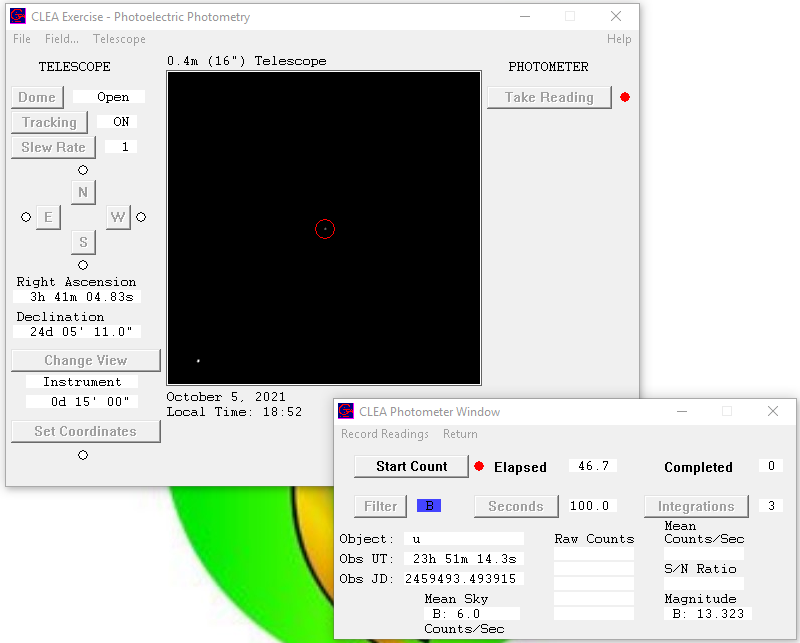
\includegraphics[width=.9\linewidth]{SMscreenshot_program.png}
    \caption{\centering Screenshot of the CLEA program in use.}
    \label{fig:program}
\end{figure}

Initial "sky" readings were taken for both filters (as seen in the separate, smaller window open in figure \ref{fig:program}) to account for the surrounding light not being emitted
from the studied star (true photon count is then \textit{star reading - sky reading}).

In addition to the \textbf{right ascension} and \textbf{declination} coordinates, which were provided, the following data was also noted and collected:

\begin{itemize}
    \item \textbf{Signal to Noise (S/N) Ratio} for both filter; fractional error.
    \item \textbf{Magnitude} (apparent) for both filters (B-V).
\end{itemize}

The uncertainties on the magnitude readings were minimised by ensuring the S/N ratio was greater than or at least 100 (70 for dimmer stars). This can be adjusted based on the amount of intergrations 
(number of times a measurement is repeated) doneand the seconds (how long light is collected for per integration) the photometer is allowed to collect data for. 

Dimmer stars generally needed more intergrations and longer seconds, with the maximum allowed to be done being: \textit{100 seconds, 5 intergrations}. This is approximately 8.5 minutes of photon collection.

With the collected data a H-R diagram can be plotted, with the apparent magnitude (V filter) and colour index (B-V), and compared against the accepted values of main sequence stars.

\section{Results and Calculations} \label{sec:3}

The data collected in the lab was put into a table (\ref{tab:1}), where B-V was calculated and the uncertainties for the S/N ratio were added in quadrature:

\vspace{-1.5ex}
\begin{gather*}
    \delta(B-V) = \sqrt{(\delta(V))^2 + (\delta(B))^2} \qquad ; \:\: \delta(V) = \frac{1}{S/R(V)} \: , \: \delta(B) = \frac{1}{S/R(B)}
\end{gather*}

\begin{table}[H]
    \centering
    \caption{\centering Table of the values gathered for the Blue (B) and Visual (V) filter with respective S/N ratios, calculated B-V and corresponding S/N ratio included.}
    \resizebox{\textwidth}{!}{

        \begin{tabular}{|c|c|c|c|c|c|c|c|c|}
        \hline
        \textbf{Star} & \textbf{\begin{tabular}[c]{@{}c@{}}RA\\ hr min sec\end{tabular}} & \textbf{\begin{tabular}[c]{@{}c@{}}Dec\\ deg min sec\end{tabular}} & \textbf{B} & \textbf{\begin{tabular}[c]{@{}c@{}}S/N\\ (B)\end{tabular}} & \textbf{V} & \textbf{\begin{tabular}[c]{@{}c@{}}S/N\\ (V)\end{tabular}} & \textbf{B-V} & \textbf{\begin{tabular}[c]{@{}c@{}}S/N\\ (B-V) (\%)\end{tabular}} \\ \hline
        \textbf{1}    & 3  41  05                                                        & 24  05  11                                                         & 13.316     & 242                                                        & 12.513     & 352                                                        & 0.80         & 0.501                                                            \\ \hline
        \textbf{2}    & 3  42  15                                                        & 24  19  57                                                         & 4.200      & 6449                                                       & 4.310      & 6130                                                       & -0.11        & 0.023                                                            \\ \hline
        \textbf{3}    & 3  42  33                                                        & 24  18  55                                                         & 8.950      & 1774                                                       & 8.600      & 2085                                                       & 0.35         & 0.074                                                            \\ \hline
        \textbf{4}    & 3  42  41                                                        & 24  28  22                                                         & 10.250     & 975                                                        & 9.699      & 1258                                                       & 0.55         & 0.130                                                            \\ \hline
        \textbf{5}    & 3  43  08                                                        & 24  42  47                                                         & 13.058     & 271                                                        & 12.048     & 352                                                        & 1.01         & 0.466                                                            \\ \hline
        \textbf{6}    & 3  43  08                                                        & 25  00  46                                                         & 15.374     & 83                                                         & 14.365     & 133                                                        & 1.01         & 1.420                                                            \\ \hline
        \textbf{7}    & 3  43  39                                                        & 23  28  58                                                         & 8.468      & 404                                                        & 8.112      & 476                                                        & 0.36         & 0.325                                                            \\ \hline
        \textbf{8}    & 3  43  42                                                        & 23  20  34                                                         & 13.007     & 226                                                        & 12.023     & 356                                                        & 0.98         & 0.524                                                            \\ \hline
        \textbf{9}    & 3  43  56                                                        & 23  25  46                                                         & 11.162     & 524                                                        & 10.522     & 498                                                        & 0.64         & 0.277                                                            \\ \hline
        \textbf{10}   & 3  44  03                                                        & 24  25  54                                                         & 6.822      & 862                                                        & 6.800      & 871                                                        & 0.02         & 0.163                                                            \\ \hline
        \textbf{11}   & 3  44  11                                                        & 24  07  23                                                         & 9.931      & 357                                                        & 9.469      & 255                                                        & 0.46         & 0.482                                                            \\ \hline
        \textbf{12}   & 3  44  19                                                        & 24  14  16                                                         & 13.782     & 80                                                         & 12.630     & 136                                                        & 1.15         & 1.450                                                            \\ \hline
        \textbf{13}   & 3  44  27                                                        & 23  57  57                                                         & 2.780      & 5547                                                       & 2.870      & 5321                                                       & -0.09        & 0.026                                                            \\ \hline
        \textbf{14}   & 3  44  39                                                        & 23  27  17                                                         & 8.952      & 723                                                        & 7.720      & 988                                                        & 1.23         & 0.171                                                            \\ \hline
        \end{tabular}
    }
    \label{tab:1}
\end{table}

\begin{table}[H]
    \centering
    \caption{\centering (Continuation) Table of the values gathered for the Blue (B) and Visual (V) filter with respective S/N ratios, calculated B-V and corresponding S/N ratio included.}
    \resizebox{\textwidth}{!}{

        \begin{tabular}{|c|c|c|c|c|c|c|c|c|}
        \hline
        \textbf{Star} & \textbf{\begin{tabular}[c]{@{}c@{}}RA\\ hr min sec\end{tabular}} & \textbf{\begin{tabular}[c]{@{}c@{}}Dec\\ deg min sec\end{tabular}} & \textbf{B} & \textbf{\begin{tabular}[c]{@{}c@{}}S/N\\ (B)\end{tabular}} & \textbf{V} & \textbf{\begin{tabular}[c]{@{}c@{}}S/N\\ (V)\end{tabular}} & \textbf{B-V} & \textbf{\begin{tabular}[c]{@{}c@{}}S/N\\ (B-V) (\%)\end{tabular}} \\ \hline
        \textbf{15}   & 3  44  39                                                        & 24  34  47                                                         & 17.032     & 79                                                         & 16.521     & 115                                                        & 0.51         & 1.536                                                            \\ \hline
        \textbf{16}   & 3  44  45                                                        & 23  24  52                                                         & 9.949      & 457                                                        & 8.802      & 775                                                        & 1.15         & 0.254                                                            \\ \hline
        \textbf{17}   & 3  45  09                                                        & 24  50  59                                                         & 8.162      & 465                                                        & 6.459      & 1018                                                       & 1.70         & 0.236                                                            \\ \hline
        \textbf{18}   & 3  45  27                                                        & 23  17  57                                                         & 5.380      & 1675                                                       & 5.450      & 1622                                                       & -0.07        & 0.086                                                            \\ \hline
        \textbf{19}   & 3  45  28                                                        & 23  53  41                                                         & 10.578     & 265                                                        & 10.018     & 343                                                        & 0.56         & 0.477                                                            \\ \hline
        \textbf{20}   & 3  45  33                                                        & 24  12  59                                                         & 7.070      & 544                                                        & 6.948      & 575                                                        & 0.12         & 0.253                                                            \\ \hline
        \textbf{21}   & 3  46  26                                                        & 23  41  11                                                         & 12.135     & 237                                                        & 11.351     & 241                                                        & 0.78         & 0.592                                                            \\ \hline
        \textbf{22}   & 3  46  26                                                        & 23  49  58                                                         & 16.807     & 82                                                         & 15.781     & 134                                                        & 1.03         & 1.430                                                            \\ \hline
        \textbf{23}   & 3  46  57                                                        & 24  04  51                                                         & 9.343      & 604                                                        & 9.168      & 507                                                        & 0.18         & 0.258                                                            \\ \hline
        \textbf{24}   & 3  47  29                                                        & 24  20  34                                                         & 7.550      & 1068                                                       & 7.421      & 655                                                        & 0.13         & 0.179                                                            \\ \hline
        \end{tabular}
    }
    \label{tab:1.5}
\end{table}

The data in table \ref{tab:1} was then graphed (figure \ref{fig:pleigraph}) with the \textbf{apparent} magnitude against the B-V magnitudes. Similar was done for data in \ref{tab:2}, but with 
the \textbf{absolute} magnitude against the B-V magnitudes (figure \ref{fig:pleimsgraph}).

\begin{figure}[H]
    \centering
    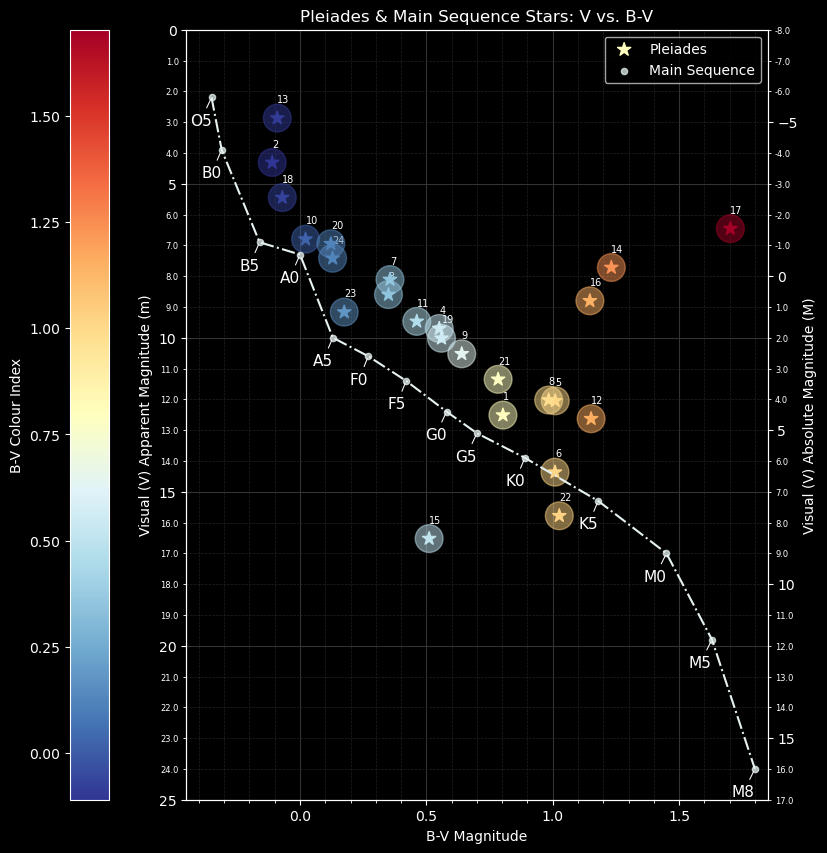
\includegraphics[width=12cm]{pleiadesms graph.png}
    \caption{\centering Graph of the Main Sequence Stars plotted against the Pleiades Cluster; \textit{individual y-axes}.}
    \label{fig:pleimsgraph}
\end{figure}

By observing figure \ref{fig:pleimsgraph} and comparing against the H-R diagram in section §\ref{sec:1.2}, figure \ref{fig:hrdiagram}, it can be concluded that the following stars could likely be red giants:

\begin{table}[H]
    \centering
    \caption{\centering Most likely red giants.}
    \begin{tabular}{p{3cm}|p{1.5cm} p{1.5cm} }
    \textbf{Star Number} & \textbf{V} & \textbf{B-V} \\
    17                   & 6.459      & 1.70         \\
    14                   & 7.720      & 1.23         \\
    16                   & 8.802      & 1.15        
    \end{tabular}
    \label{tab:3}
\end{table}

Observing figure \ref{fig:pleimsgraph} again, Star No.15's divergence away from the rest of the star cluster is examined. According to the Main Sequence trail included,
it would be of spectral class G, which is the same class our Sun belongs to so it can be assumed Star No.15 would be of \textbf{similar yellow-white colour} and likely between the same temperatures of 4 900–5 700 K. 
However, given its isolation from the rest of the Pleiades star cluster this is likely not as prominent as its sisters.

\subsection{Distance to the Pleiades Star Cluster Calculations} \label{sec:3.1}

The distance to the cluster from Earth in parsecs can be found using equation \ref{eq:2}. In the case of this experiment as the absolute magnitudes were not calculated the error on the distance is entirely tied 
to the error on the apparent magnitudes found. A derivation of the equation \ref{eq:2} must then be performed.

As was covered in sections §\ref{sec:1.1.3.1} and §\ref{sec:1.1.3.2}, the formula for the apparent magnitude depedent on flux is such:

\vspace{-1.5ex}
\begin{gather*}
    m = -2.5 \log_{10}(F)
\end{gather*}

And the error on \textit{m} is found by its derivative:

\vspace{-1.5ex}
\begin{gather} \label{eq:5}
    \frac{d}{dx} \log_ax = \frac{1}{x\ln a}dx \qquad \implies \qquad \Delta m = - \frac{2.5}{\ln 10}\frac{dF}{F}
\end{gather}

But with the signal to noise (S/N) ratio being defined as the following,

\vspace{-1.5ex}
\begin{gather*}
    S/R = \frac{F}{dF}
\end{gather*}

It can be observed how equation \ref{eq:5} contains $S/R^{-1}$. As such, the error does not need to be propagated due to the presence of only one variable, giving it a strict y dependence.
With this knowledge, equation \ref{eq:2} can now be differentiated with respect to \textit{m} as a total derivative and multiplied by the error on \textit{m}:

\vspace{-1.5ex}
\begin{gather*}
    \Delta D = \left( \frac{d}{dm} 10^{\frac{m - M + 5}{5}} \right) \cdot \Delta m
\end{gather*}

The following can then be used,

\vspace{-1.5ex}
\begin{gather*}
    \frac{d}{dx}10^{x} = 10^{x} \ln(10)
\end{gather*}

To obtain from the previous equation:

\vspace{-1.5ex}
\begin{gather*}
    \Delta D = \left( \frac{1}{5} 10^{\frac{m-M+5}{5}} \right) \left( \ln 10 \right) \Delta m
\end{gather*}

With the $\Delta m$ from equation \ref{eq:5}, the result is then:

\vspace{-1.5ex}
\begin{gather*}
    \Delta D = \left( \frac{1}{\cancel{5}2} 10^{\frac{m-M+5}{5}} \right) (\cancel{\ln 10}) \frac{\cancel{2.5}}{\cancel{\ln 10}} \cdot \frac{dF}{F}
\end{gather*}

So finally the error on the distance is as follows \cite{rian}:

\vspace{-1.5ex}
\begin{gather}
    \Delta D = \frac{10^{\frac{m-M+5}{5}}}{2 \cdot S/R} \quad = \quad \frac{D}{2 \cdot S/R}
\end{gather}

The distance can be calculated once the absolute magnitude and its corresponding apparent magnitude are found, which was done by locating the area on the simulated
H-R diagram where the main sequence meets the Giants region (the bend) \cite{dist}. The magnitude values were approximated to be \textbf{M = 4.75, m = 10.25} from figure \ref{fig:adjgraph}. These can be substituted
into the equations below, with the distance modulus (m - M) equal to \textbf{5.5}.

\begin{gather*}
    D = 10 \times 10^{\frac{10.25-4.75}{5}} \quad\quad \Delta D = \frac{D}{2 (\text{average}(S/R(V)))}
\end{gather*}

The code for this calculation can be found in the Appendix (§\ref{sec:A}). The distance \textbf{D} is found to be \textbf{125.8925 pc}. The values above are then multiplied by \textbf{3.26} to \textbf{convert from parsecs (pc) to light-years (ly)}.
The final calculated distance to the Pleiades from Earth is $\mathbf{410.4097 \pm 0.1955}$ \textbf{ly}.

This value is a \textbf{0.0999\%} difference to the value of 410 ly calculated by \textit{H.L. Johnson and R.I. Mitchell} in 1958 and a \textbf{6.7251\%} difference to the value of 440 ly calculated by 
\textit{NASA/ESA Hubble Telescope} in 2004 (see §\ref{sec:1.3}).

\subsection{The Apparent Magnitude of the Sun} \label{sec:3.2}

Below, figure \ref{fig:sunfeature}, the Sun has been plotted along the Main Sequence line (as the Sun belongs to the Main Sequence) at its respective B-V value, \textbf{+0.62}.

\begin{figure}[H]
    \centering
    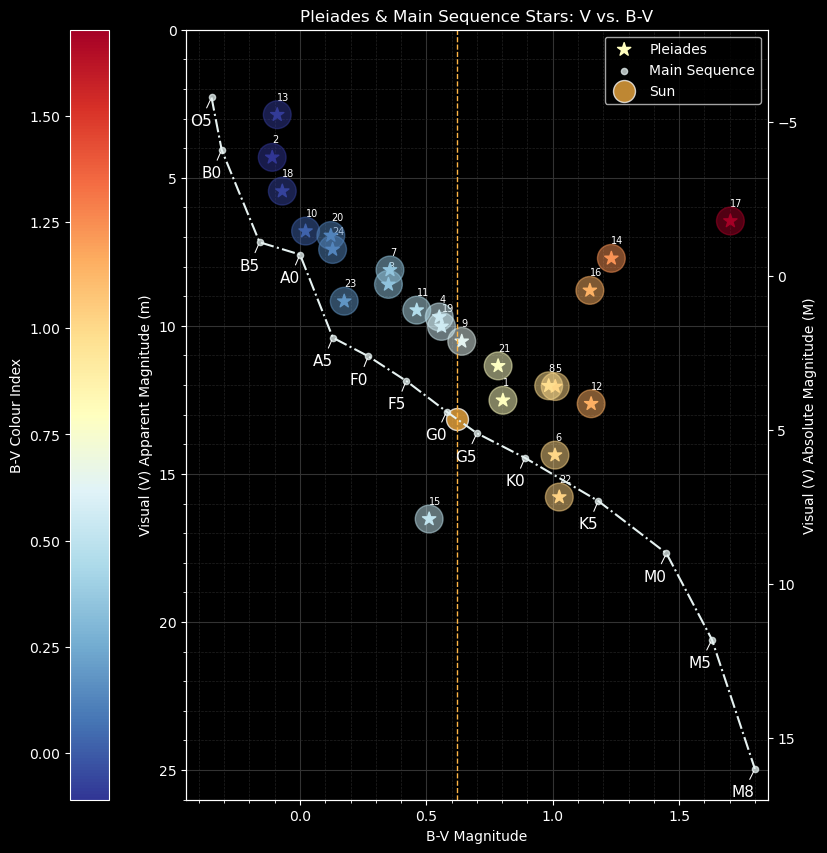
\includegraphics[width=12.5cm]{pleimsgraph sun.png}
    \caption{\centering figure \ref{fig:pleimsgraph} with Sun position labelled; axes adjusted to align Main Sequence to Pleiades.}
    \label{fig:sunfeature}
\end{figure}

The \textit{absolute magnitude} for the Sun is found to be \textbf{4.63} from the graph, which is only 0.20 (4.14\%) different from the accepted value of \textbf{4.83} \cite{sun}.
By further observation of the graph it can be found that the \textit{apparent magnitude} of the Sun (if it were part of the Pleiades cluster) would be approximately \textbf{10.25}.
The \textit{apparent magnitude} can also be found by using the distance formula (equation \ref{eq:1}):

\begin{gather*}
    m = M - 5 + 5 \log_{10} (D) \quad \implies \quad m = 4.63 -5 + 5 \log_{10}(125.8925)
\end{gather*}

The result is an apparent magnitude of \textbf{10.13}. This is a 1.177\% difference, with the manually computed method more accurate than the estimation through observation.

The distance modulus (m - M) with these values, taking the manually computed apparent magnitude, is then found to be \textbf{5.5}. This is the same value as calculated for section §\ref{sec:3.1}.
The consistency in this value suggests that the distance calculated in section §\ref{sec:3.1} is \textit{internally} consistent within the confines of this experiment, not necessarily that the actual
distance to the Pleiades is 410 ly as calculated.

\newpage

\section{Conclusion} \label{sec:4}

The experiment was successful in its use of the photometer and photometric measurements to calculate the distance to the Pleiades star cluster.
Through the analysis of the apparent magnitudes of the 24 pre-determined stars within the cluster for a blue (B) and visual (V) filter values for the B-V colour index were found to be 
between \textbf{-0.11 and 1.70}. These values allowed for the graphing of the V apparent magnitude against the B-V values, as seen in figure \ref{fig:pleigraph}. The Main Sequence line as seen in the 
H-R diagram (figure \ref{fig:hrdiagram}) was plotted also (see figure \ref{fig:msgraph}) and the two graphs were replotted as one (see figure \ref{fig:pleimsgraph}).

This graph allowed for the calculation of the distance modulus, resulting as \textbf{0.55}, and the distance to the Pleiades cluster with its uncertainty both in lightyears, $\mathbf{410.4097 \pm 0.1955}$ \textbf{ly}.
This value was a \textbf{0.0999\%} difference to the value calculated in 1958 by \textit{H.L. Johnson and R.I. Mitchell} (410 ly) and a \textbf{6.721\%} difference to the value
calculated in 2004 by the \textit{NASA/ESA Hubble Telescope} (440 ly).

The distance to the Sun as if it were in the Pleiades was then considered as a consistency check as it is known that the Sun lies on the Main Sequence line. By finding the point of intersection
at this line from the known Sun B-V value of \textbf{+0.62} the apparent and absolute magnitudes could be assumed from reading the graph (see figure \ref{fig:sunfeature}). The distance modulus was found
again to be \textbf{0.55} and the discrepancy between the two estimated values of the apparent magnitude to be \textbf{1.177\%}. This suggests that the values are consistent within the experiment; the experiment would need to
be expanded further in order to align with real-world values.

For future renditions of this experiment iterations and seconds could be managed better to further reduce the signal to noise ratio and therefore errors on the values.
Any values that were "eyeballed" (such as Sun magnitudes, Pleiades magnitudes, for distance calculations) could be refined with more code to get exact values, but due to time constraints
this was not feasible. There is, therefore, the error of parallax in regard to these measurements.

\newpage

%%%%%%%%%%%%%%%%%%%%%%%%%%%%%%%%%%%

\bibliographystyle{IEEEtran}
\bibliography{References} \label{sec:ref}

\vspace{1.5cm}

\listoffigures

\listoftables

\section*{Appendix} \label{sec:A}
\addcontentsline{toc}{section}{Appendix}

\subsection*{Tables}
\addcontentsline{toc}{subsection}{Tables}

\begin{table}[H]
    \centering
    \caption{\centering Table of the Sky Reading measurements taken before official experiment.}

    \begin{tabular}{c||c}
    \textbf{Filter} & \textbf{Mean Sky (Counts/sec)} \\
    \textbf{B}      & 6.0                            \\
    \textbf{V}      & 16.6                          
    \end{tabular}
\end{table}

\begin{table}[H]
    \centering
    \caption{\centering Table of the provided data for the main sequence stars to be plotted \protect\cite{UCDsm, cleasm}.}

    \begin{tabular}{|c|c|c|}
    \hline
    \textbf{\begin{tabular}[c]{@{}c@{}}(V) Absolute\\ Magnitude\end{tabular}} & \textbf{B-V} & \textbf{Spectral Type} \\ \hline
    -5.8                                                                      & -0.35        & O5                     \\ \hline
    -4.1                                                                      & -0.31        & B0                     \\ \hline
    -1.1                                                                      & -0.16        & B5                     \\ \hline
    -0.7                                                                      & 00.0         & A0                     \\ \hline
    2.0                                                                       & 0.13         & A5                     \\ \hline
    2.6                                                                       & 0.27         & F0                     \\ \hline
    3.4                                                                       & 0.42         & F5                     \\ \hline
    4.4                                                                       & 0.58         & G0                     \\ \hline
    5.1                                                                       & 0.70         & G5                     \\ \hline
    5.9                                                                       & 0.89         & K0                     \\ \hline
    7.3                                                                       & 1.18         & K5                     \\ \hline
    9.0                                                                       & 1.45         & M0                     \\ \hline
    11.8                                                                      & 1.63         & M5                     \\ \hline
    16.0                                                                      & 1.80         & M8                     \\ \hline
    \end{tabular}
    \label{tab:2}
\end{table}

\subsection*{Graphs}
\addcontentsline{toc}{subsection}{Graphs}

\begin{minipage}{.49\textwidth}
    \captionsetup{hypcap=false}
    \centering
    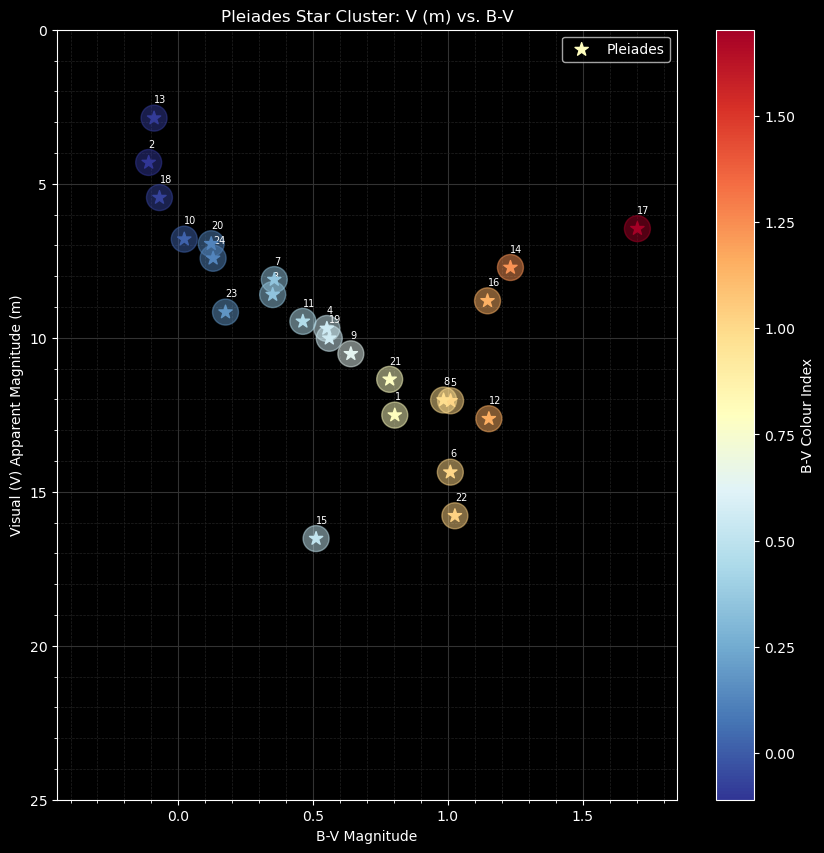
\includegraphics[width=\linewidth]{pleiades graoh.png}
    \captionof{figure}{\centering Graph of the Pleiades data.}
    \label{fig:pleigraph}
\end{minipage}
\hfill
\begin{minipage}{.5\textwidth}
    \captionsetup{hypcap=false}
    \centering
    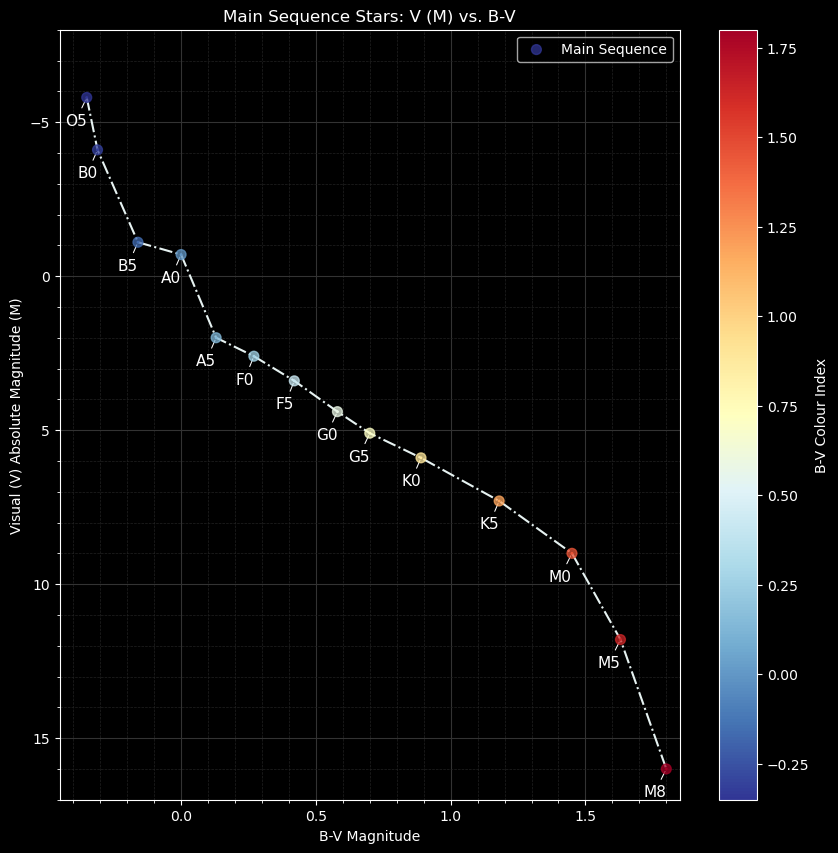
\includegraphics[width=\linewidth]{ms graph.png}
    \captionof{figure}{\centering Graph of Main Sequence stars.}
    \label{fig:msgraph}
\end{minipage}

\begin{figure}[H]
    \centering
    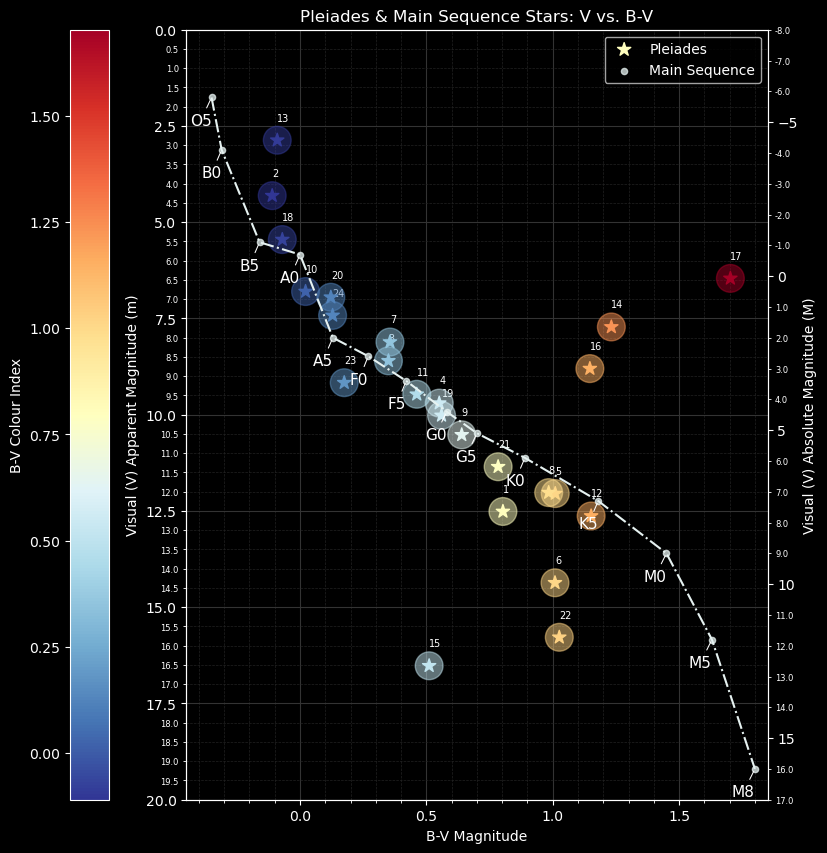
\includegraphics[width=12.5cm]{20 axis pleims.png}
    \caption{\centering figure \ref{fig:pleimsgraph} with adjusted axes such that Main Sequence aligns with the Pleiades star cluster.}
    \label{fig:adjgraph}
\end{figure}

\subsection*{Code}
\addcontentsline{toc}{subsection}{Code}

%

\begin{minipage}{\linewidth}
\captionsetup{hypcap=false}

\begin{mintedbox}
\begin{minted}[fontsize=\small, breaklines, baselinestretch=1.2, xleftmargin=0.5cm]{python}
import numpy as np
import matplotlib.pyplot as plt

def errorprop(dx, dy): # error propagation defined formula
    error_x = 1 / dx
    error_y = 1 / dy

    return np.sqrt(error_x**2 + error_y**2)

B = np.array([13.316, 4.200, 8.950, 10.250, 13.058, 15.374, 8.468, 13.007, 11.162, 6.822, 9.931, 13.782, 2.780, 8.952, 17.032, 9.949, 8.162, 5.380, 10.578, 7.070, 12.135, 16.807, 9.343, 7.550])
sn_B = np.array([242, 6449, 1774, 975, 271, 83, 404, 226, 524, 862, 357, 80, 5547, 723, 79, 457, 465, 1675, 265, 544, 237, 82, 604, 1068])
V = np.array([12.513, 4.310, 8.600, 9.699, 12.048, 14.365, 8.112, 12.023, 10.522, 6.800, 9.469, 12.630, 2.870, 7.720, 16.521, 8.802, 6.459, 5.450, 10.018, 6.948, 11.351, 15.781, 9.168, 7.421])
sn_V = np.array([352, 6130, 2085, 1258, 352, 133, 476, 356, 498, 871, 255, 136, 5321, 988, 115, 775, 1018, 1622, 343, 575, 241, 134, 507, 655])
print(B-V)
print(errorprop(sn_B,sn_V)) # fractional error, since they're already put into fractions in the eqn
print(errorprop(sn_B,sn_V)*100) # percentage error

\end{minted}
\end{mintedbox}

\captionof{figure}{\centering Code used for table \ref{tab:1} in calculating the S/N ratio for B-V.}
\end{minipage}

\begin{minipage}{\linewidth}
\captionsetup{hypcap=false}

\begin{mintedbox}
\begin{minted}[fontsize=\small, breaklines, baselinestretch=1.2, xleftmargin=0.5cm]{python}
m_approx = 10.25
M_approx = 4.75

def D_func(m, M):
    D_mod = m - M
    D1 = 10**((D_mod)/5)
    return (10*D1)
print(D_func(m_approx, M_approx) * 3.26) # D in ly

def D_err(D, SR):
    return (D/(2*SR))
print(D_err(D_func(m_approx, M_approx), np.average(sn_V)) * 3.26) # err on D in ly

\end{minted}
\end{mintedbox}

\captionof{figure}{\centering Code used for section §\ref{sec:3.1} calculations.}
\end{minipage}

\begin{minipage}{\linewidth}
\captionsetup{hypcap=false}

\begin{mintedbox}
\begin{minted}[fontsize=\small, breaklines, baselinestretch=1.2, xleftmargin=0.5cm]{python}
plt.figure(figsize=(10,10))

# Plot
plt.scatter(BV, V, c=BV, cmap='RdYlBu_r', alpha=0.5, zorder=3, s=350)
plt.scatter(BV, V, c=BV, cmap='RdYlBu_r', zorder=4, s=100, marker="*", label="Pleiades")

#Grid
plt.minorticks_on()
plt.grid(True, which="major", linewidth=0.8, color="#333333", zorder=2)
plt.grid(True, which="minor", linewidth=0.5, color="#222222", linestyle="--", zorder=1)
plt.ylim(0,25)
plt.xlim(-0.45,1.85)
plt.gca().invert_yaxis()

# Style
plt.style.use('dark_background')
plt.colorbar(label="B-V Colour Index")

# Labels
plt.title("Pleiades Star Cluster: V (m) vs. B-V")
plt.xlabel("B-V Magnitude")
plt.ylabel("Visual (V) Apparent Magnitude (m)")
plt.legend()

plt.show()

\end{minted}
\end{mintedbox}

\captionof{figure}{\centering Code used for figure \ref{fig:pleigraph}.}
\end{minipage}

\begin{minipage}{\linewidth}
\captionsetup{hypcap=false}

\begin{mintedbox}
\begin{minted}[fontsize=\small, breaklines, baselinestretch=1.2, xleftmargin=0.5cm]{python}
BV_ms = np.array([-0.35, -0.31, -0.16, 00.0, 0.13, 0.27, 0.42, 0.58, 0.70, 0.89, 1.18, 1.45, 1.63, 1.80])
V_ms =  np.array([-5.8, -4.1, -1.1, -0.7, 2.0, 2.6, 3.4, 4.4, 5.1, 5.9, 7.3, 9.0, 11.8, 16.0])

spectral_type = ["O5", "B0", "B5", "A0", "A5", "F0", "F5", "G0", "G5", "K0", "K5", "M0", "M5", "M8"]

# Plot
fig, ax = plt.subplots(figsize=(10,10))

plt.plot(BV_ms, V_ms, c="#e6f2f1", zorder=3, linestyle="-.")
plt.scatter(BV_ms, V_ms, c=BV_ms, cmap="RdYlBu_r", alpha=0.75, s=50, zorder=4, label="Main Sequence")
plt.scatter(BV_ms, V_ms, c=BV_ms, cmap="RdYlBu_r", s=1, zorder=8)

# Style
plt.style.use('dark_background')
plt.colorbar(label="B-V Colour Index")

# Grid
plt.minorticks_on()
plt.grid(True, which="major", linewidth=0.8, color="#333333", zorder=2)
plt.grid(True, which="minor", linewidth=0.5, color="#222222", linestyle="--", zorder=1)
plt.ylim(-8,17)
plt.xlim(-0.45,1.85)
plt.gca().invert_yaxis()

# Spectral Type Labels (Main Sequence) 
for i in range(len(BV_ms)): # credit to Mr. ChatGPT
    ax.annotate(
        spectral_type[i],
        xy = (BV_ms[i], V_ms[i]),
        xytext = (BV_ms[i], V_ms[i] + 0.9),
        color="white", fontsize=11, ha="right", zorder=3,
        arrowprops=dict(arrowstyle="-", color="white", lw=0.75)
    )

\end{minted}
\end{mintedbox}

\captionof{figure}{\centering Code used for figure \ref{fig:msgraph}.}
\end{minipage}

\begin{minipage}{\linewidth}
\captionsetup{hypcap=false}

\begin{mintedbox}
\begin{minted}[fontsize=\small, breaklines, baselinestretch=1.2, xleftmargin=0.5cm]{python}
# Labels
plt.title("Main Sequence Stars: V (M) vs. B-V")
plt.xlabel("B-V Magnitude")
plt.ylabel("Visual (V) Absolute Magnitude (M)")
plt.legend()

plt.show()

\end{minted}
\end{mintedbox}

\captionof{figure}{\centering Continuation of the code used for figure \ref{fig:msgraph}.}
\end{minipage}

%

\begin{minipage}{\linewidth}
\captionsetup{hypcap=false}

\begin{mintedbox}
\begin{minted}[fontsize=\small, breaklines, baselinestretch=1.2, xleftmargin=0.5cm]{python}
# Pleiades
fig, ax1 = plt.subplots(figsize=(10,10))
ax1.set_axisbelow(True)

ax1.scatter(BV, V, c=BV, cmap="RdYlBu_r", alpha=0.5, s=400, zorder=6)
plei_sc = ax1.scatter(BV, V, c=BV, cmap="RdYlBu_r", s=100, marker="*", label="Pleiades", zorder=7)

plei_cbar = fig.colorbar(plei_sc, ax=ax1, label="B-V Colour Index", location="left")

ax1.set_ylim(26,0.0)
ax1.set_ylabel("Visual (V) Apparent Magnitude (m)")
ax1.tick_params(axis="y")

# Shared bit (x-axis)
ax1.set_xlim(-0.45,1.85)
ax1.set_xlabel("B-V Magnitude")

\end{minted}
\end{mintedbox}

\captionof{figure}{\centering Code used for figure \ref{fig:pleimsgraph}.}
\end{minipage}

\begin{minipage}{\linewidth}
\captionsetup{hypcap=false}

\begin{mintedbox}
\begin{minted}[fontsize=\small, breaklines, baselinestretch=1.2, xleftmargin=0.5cm]{python}
# Main Sequence
ax2 = ax1.twinx()
ax2.set_axisbelow(True)

ax2.plot(BV_ms, V_ms, c="#e6f2f1", zorder=3, linestyle="-.")
ax2.scatter(BV_ms, V_ms, c="#e6f2f1", alpha=0.75, s=20, zorder=2, label="Main Sequence")

ax2.set_ylim(17,-8)
ax2.set_ylabel("Visual (V) Absolute Magnitude (M)")
ax2.tick_params(axis="y")

# Grids
ax1.minorticks_on()
ax1.grid(True, which="major", linewidth=0.8, color="#333333", zorder=0)  # Major grid
ax1.grid(True, which="minor", linewidth=0.5, color="#222222", linestyle="--", zorder=0)  # Minor grid

# Spectral Type Labels (Main Sequence)
for i in range(len(BV_ms)): # credit to Mr. ChatGPT
    ax2.annotate(
        spectral_type[i],
        xy = (BV_ms[i], V_ms[i]),
        xytext = (BV_ms[i], V_ms[i] + 0.9),
        color="white", fontsize=11, ha="right", zorder=7,
        arrowprops=dict(arrowstyle="-", color="white", lw=0.75)
    )

# Star Number
for i in range(len(BV)): # credit to Mr. ChatGPT
    ax1.annotate(
        star_no[i],
        xy = (BV[i], V[i]),
        xytext = (BV[i], V[i] - 0.5),
        color="white", fontsize=7, ha="left", zorder=3,
    )

# Style
plt.style.use("dark_background")

\end{minted}
\end{mintedbox}

\captionof{figure}{\centering Continuation of the code used for figure \ref{fig:pleimsgraph}.}
\end{minipage}

\begin{minipage}{\linewidth}
\captionsetup{hypcap=false}

\begin{mintedbox}
\begin{minted}[fontsize=\small, breaklines, baselinestretch=1.2, xleftmargin=0.5cm]{python}
# Labels
plt.title("Pleiades & Main Sequence Stars: V vs. B-V")
handles1, labels1 = ax1.get_legend_handles_labels()
handles2, labels2 = ax2.get_legend_handles_labels()
ax1.legend(handles1 + handles2, labels1 + labels2, loc="upper right")

fig.canvas.draw()

plt.show()

\end{minted}
\end{mintedbox}

\captionof{figure}{\centering Continuation of the code used for figure \ref{fig:pleimsgraph}.}
\end{minipage}

\begin{minipage}{\linewidth}
\captionsetup{hypcap=false}

\begin{mintedbox}
\begin{minted}[fontsize=\small, breaklines, baselinestretch=1.2, xleftmargin=0.5cm]{python}
# Plot Sun
x = 0.62
y = np.interp(x, BV_ms, V_ms)

plt.axvline(x=0.62, color="#ffb545", linestyle="--", linewidth="1")
plt.scatter([x],[y], color="#ffb545", edgecolor="white", s=250, alpha=0.75, label="Sun")
\end{minted}
\end{mintedbox}

\captionof{figure}{\centering Code used for plotting Sun on the Main Sequence line in figure \ref{fig:sunfeature}.}
\end{minipage}

\begin{minipage}{\linewidth}
\captionsetup{hypcap=false}

\begin{mintedbox}
\begin{minted}[fontsize=\small, breaklines, baselinestretch=1.2, xleftmargin=0.5cm]{python}
from matplotlib.ticker import AutoMinorLocator, FormatStrFormatter

ax1.yaxis.set_minor_locator(AutoMinorLocator())
ax1.yaxis.set_minor_formatter(FormatStrFormatter("%.1f")) 
ax2.yaxis.set_minor_locator(AutoMinorLocator())  # Adjust minor tick placement (ChatGPT credit)
ax2.yaxis.set_minor_formatter(FormatStrFormatter("%.1f"))  # Format as 1 decimal place (ChatGPT credit)

# Force Matplotlib to display minor tick labels (ChatGPT credit)
ax1.tick_params(axis='y', which='minor', labelsize=6)
ax2.tick_params(axis='y', which='minor', labelsize=6)

\end{minted}
\end{mintedbox}

\captionof{figure}{\centering Code added to figure \ref{fig:pleimsgraph} to add numbers to the minorticks to make reading the graph easier.}
\end{minipage}

\end{document}